% Options for packages loaded elsewhere
\PassOptionsToPackage{unicode}{hyperref}
\PassOptionsToPackage{hyphens}{url}
%
\documentclass[
  ngerman,
  ignorenonframetext,
]{beamer}
\usepackage{pgfpages}
\setbeamertemplate{caption}[numbered]
\setbeamertemplate{caption label separator}{: }
\setbeamercolor{caption name}{fg=normal text.fg}
\beamertemplatenavigationsymbolsempty
% Prevent slide breaks in the middle of a paragraph
\widowpenalties 1 10000
\raggedbottom
\setbeamertemplate{part page}{
  \centering
  \begin{beamercolorbox}[sep=16pt,center]{part title}
    \usebeamerfont{part title}\insertpart\par
  \end{beamercolorbox}
}
\setbeamertemplate{section page}{
  \centering
  \begin{beamercolorbox}[sep=12pt,center]{part title}
    \usebeamerfont{section title}\insertsection\par
  \end{beamercolorbox}
}
\setbeamertemplate{subsection page}{
  \centering
  \begin{beamercolorbox}[sep=8pt,center]{part title}
    \usebeamerfont{subsection title}\insertsubsection\par
  \end{beamercolorbox}
}
\AtBeginPart{
  \frame{\partpage}
}
\AtBeginSection{
  \ifbibliography
  \else
    \frame{\sectionpage}
  \fi
}
\AtBeginSubsection{
  \frame{\subsectionpage}
}
\usepackage{amsmath,amssymb}
\usepackage{lmodern}
\usepackage{iftex}
\ifPDFTeX
  \usepackage[T1]{fontenc}
  \usepackage[utf8]{inputenc}
  \usepackage{textcomp} % provide euro and other symbols
\else % if luatex or xetex
  \usepackage{unicode-math}
  \defaultfontfeatures{Scale=MatchLowercase}
  \defaultfontfeatures[\rmfamily]{Ligatures=TeX,Scale=1}
\fi
\usetheme[]{Berkeley}
% Use upquote if available, for straight quotes in verbatim environments
\IfFileExists{upquote.sty}{\usepackage{upquote}}{}
\IfFileExists{microtype.sty}{% use microtype if available
  \usepackage[]{microtype}
  \UseMicrotypeSet[protrusion]{basicmath} % disable protrusion for tt fonts
}{}
\makeatletter
\@ifundefined{KOMAClassName}{% if non-KOMA class
  \IfFileExists{parskip.sty}{%
    \usepackage{parskip}
  }{% else
    \setlength{\parindent}{0pt}
    \setlength{\parskip}{6pt plus 2pt minus 1pt}}
}{% if KOMA class
  \KOMAoptions{parskip=half}}
\makeatother
\usepackage{xcolor}
\IfFileExists{xurl.sty}{\usepackage{xurl}}{} % add URL line breaks if available
\IfFileExists{bookmark.sty}{\usepackage{bookmark}}{\usepackage{hyperref}}
\hypersetup{
  pdftitle={Thema 1: Was ist Inferenzstatistik?},
  pdfauthor={Prof.~Sauer},
  pdflang={de-DE},
  hidelinks,
  pdfcreator={LaTeX via pandoc}}
\urlstyle{same} % disable monospaced font for URLs
\newif\ifbibliography
\usepackage{color}
\usepackage{fancyvrb}
\newcommand{\VerbBar}{|}
\newcommand{\VERB}{\Verb[commandchars=\\\{\}]}
\DefineVerbatimEnvironment{Highlighting}{Verbatim}{commandchars=\\\{\}}
% Add ',fontsize=\small' for more characters per line
\usepackage{framed}
\definecolor{shadecolor}{RGB}{248,248,248}
\newenvironment{Shaded}{\begin{snugshade}}{\end{snugshade}}
\newcommand{\AlertTok}[1]{\textcolor[rgb]{0.94,0.16,0.16}{#1}}
\newcommand{\AnnotationTok}[1]{\textcolor[rgb]{0.56,0.35,0.01}{\textbf{\textit{#1}}}}
\newcommand{\AttributeTok}[1]{\textcolor[rgb]{0.77,0.63,0.00}{#1}}
\newcommand{\BaseNTok}[1]{\textcolor[rgb]{0.00,0.00,0.81}{#1}}
\newcommand{\BuiltInTok}[1]{#1}
\newcommand{\CharTok}[1]{\textcolor[rgb]{0.31,0.60,0.02}{#1}}
\newcommand{\CommentTok}[1]{\textcolor[rgb]{0.56,0.35,0.01}{\textit{#1}}}
\newcommand{\CommentVarTok}[1]{\textcolor[rgb]{0.56,0.35,0.01}{\textbf{\textit{#1}}}}
\newcommand{\ConstantTok}[1]{\textcolor[rgb]{0.00,0.00,0.00}{#1}}
\newcommand{\ControlFlowTok}[1]{\textcolor[rgb]{0.13,0.29,0.53}{\textbf{#1}}}
\newcommand{\DataTypeTok}[1]{\textcolor[rgb]{0.13,0.29,0.53}{#1}}
\newcommand{\DecValTok}[1]{\textcolor[rgb]{0.00,0.00,0.81}{#1}}
\newcommand{\DocumentationTok}[1]{\textcolor[rgb]{0.56,0.35,0.01}{\textbf{\textit{#1}}}}
\newcommand{\ErrorTok}[1]{\textcolor[rgb]{0.64,0.00,0.00}{\textbf{#1}}}
\newcommand{\ExtensionTok}[1]{#1}
\newcommand{\FloatTok}[1]{\textcolor[rgb]{0.00,0.00,0.81}{#1}}
\newcommand{\FunctionTok}[1]{\textcolor[rgb]{0.00,0.00,0.00}{#1}}
\newcommand{\ImportTok}[1]{#1}
\newcommand{\InformationTok}[1]{\textcolor[rgb]{0.56,0.35,0.01}{\textbf{\textit{#1}}}}
\newcommand{\KeywordTok}[1]{\textcolor[rgb]{0.13,0.29,0.53}{\textbf{#1}}}
\newcommand{\NormalTok}[1]{#1}
\newcommand{\OperatorTok}[1]{\textcolor[rgb]{0.81,0.36,0.00}{\textbf{#1}}}
\newcommand{\OtherTok}[1]{\textcolor[rgb]{0.56,0.35,0.01}{#1}}
\newcommand{\PreprocessorTok}[1]{\textcolor[rgb]{0.56,0.35,0.01}{\textit{#1}}}
\newcommand{\RegionMarkerTok}[1]{#1}
\newcommand{\SpecialCharTok}[1]{\textcolor[rgb]{0.00,0.00,0.00}{#1}}
\newcommand{\SpecialStringTok}[1]{\textcolor[rgb]{0.31,0.60,0.02}{#1}}
\newcommand{\StringTok}[1]{\textcolor[rgb]{0.31,0.60,0.02}{#1}}
\newcommand{\VariableTok}[1]{\textcolor[rgb]{0.00,0.00,0.00}{#1}}
\newcommand{\VerbatimStringTok}[1]{\textcolor[rgb]{0.31,0.60,0.02}{#1}}
\newcommand{\WarningTok}[1]{\textcolor[rgb]{0.56,0.35,0.01}{\textbf{\textit{#1}}}}
\usepackage[normalem]{ulem}
% Avoid problems with \sout in headers with hyperref
\pdfstringdefDisableCommands{\renewcommand{\sout}{}}
\setlength{\emergencystretch}{3em} % prevent overfull lines
\providecommand{\tightlist}{%
  \setlength{\itemsep}{0pt}\setlength{\parskip}{0pt}}
\setcounter{secnumdepth}{-\maxdimen} % remove section numbering
%\setbeamertemplate{page number in head/foot}[totalframenumber]
\setbeamertemplate{footline}[frame number]
\ifXeTeX
  % Load polyglossia as late as possible: uses bidi with RTL langages (e.g. Hebrew, Arabic)
  \usepackage{polyglossia}
  \setmainlanguage[]{german}
\else
  \usepackage[main=ngerman]{babel}
% get rid of language-specific shorthands (see #6817):
\let\LanguageShortHands\languageshorthands
\def\languageshorthands#1{}
\fi
\ifLuaTeX
  \usepackage{selnolig}  % disable illegal ligatures
\fi
\newlength{\cslhangindent}
\setlength{\cslhangindent}{1.5em}
\newlength{\csllabelwidth}
\setlength{\csllabelwidth}{3em}
\newenvironment{CSLReferences}[2] % #1 hanging-ident, #2 entry spacing
 {% don't indent paragraphs
  \setlength{\parindent}{0pt}
  % turn on hanging indent if param 1 is 1
  \ifodd #1 \everypar{\setlength{\hangindent}{\cslhangindent}}\ignorespaces\fi
  % set entry spacing
  \ifnum #2 > 0
  \setlength{\parskip}{#2\baselineskip}
  \fi
 }%
 {}
\usepackage{calc}
\newcommand{\CSLBlock}[1]{#1\hfill\break}
\newcommand{\CSLLeftMargin}[1]{\parbox[t]{\csllabelwidth}{#1}}
\newcommand{\CSLRightInline}[1]{\parbox[t]{\linewidth - \csllabelwidth}{#1}\break}
\newcommand{\CSLIndent}[1]{\hspace{\cslhangindent}#1}

\title{Thema 1: Was ist Inferenzstatistik?}
\subtitle{QM2, ROS, Kap. 1,}
\author{Prof.~Sauer}
\date{WiSe 21}
\institute{AWM, HS Ansbach}

\begin{document}
\frame{\titlepage}

\begin{frame}[allowframebreaks]
  \tableofcontents[hideallsubsections]
\end{frame}
\hypertarget{was-ist-inferenzstatistik}{%
\section{Was ist Inferenzstatistik?}\label{was-ist-inferenzstatistik}}

\begin{frame}{Deskriptiv- vs.~Inferenzstatistik}
\protect\hypertarget{deskriptiv--vs.-inferenzstatistik}{}
\begin{figure}[H]
\includegraphics[width=0.7\linewidth]{/Users/sebastiansaueruser/Google Drive/research/Publikationen/In_Arbeit/Statistik__21/images/Rahmen/desk_vs_inf} \end{figure}
\end{frame}

\begin{frame}{Wozu ist die Inferenstatistik da?}
\protect\hypertarget{wozu-ist-die-inferenstatistik-da}{}
\begin{alertblock}{Definition}
Inferenzstatistik ist ein Verfahren, das mathematische Modelle verwendet, um von einer bestimmten Datenlage, die eine Stichprobe einer Grundgesamtheit darstellt, allgemeine Schlüsse zu ziehen.
\end{alertblock}
\end{frame}

\begin{frame}{Die drei Aufgaben der Inferenzstatistik}
\protect\hypertarget{die-drei-aufgaben-der-inferenzstatistik}{}
\begin{enumerate}
\item
  Von der Stichprobe auf die Grundgesamtheit schließen
\item
  Von der Experimental- auf die Kontrollgruppe zu schließen
\item
  Vom beobachteten Messwert auf das zugrundeliegende Konstrukt zu
  schließen
\end{enumerate}
\end{frame}

\begin{frame}{Deskriptiv- und Inferenzstatistik gehen Hand in Hand}
\protect\hypertarget{deskriptiv--und-inferenzstatistik-gehen-hand-in-hand}{}
Für jede Kennzahl der Deskriptivstatistik (d.h. Stichprobendaten) kann
man die Methoden der Inferenzstatistik verwenden (auf eine
Grundgesamtheit schließen), z.B.:

\begin{table}
\centering
\begin{tabular}{l|l|l}
\hline
Kennwert & Stichprobe & Grundgesamtheit\\
\hline
Mittelwert & $\bar{X}$ & $\mu$\\
\hline
Streuung & $sd$ & $\sigma$\\
\hline
Anteil & $p$ & $\pi$\\
\hline
Korrelation & $r$ & $\rho$\\
\hline
Regression & $b$ & $\beta$\\
\hline
\end{tabular}
\end{table}

Für Stichprobendaten verwendet man lateinische Buchstaben
(\(X, p, b, \ldots\)); für Populationsdaten verwendet man griechische
Buchstaben.
\end{frame}

\begin{frame}{Schätzen von Parametern einer Grundgesamtheit}
\protect\hypertarget{schuxe4tzen-von-parametern-einer-grundgesamtheit}{}
Meist begnügt man sich nicht mit Aussagen für eine Stichprobe, sondern
will auf eine Grundgesamtheit verallgemeinern.

Leider sind die Parameter einer Grundgesamtheit zumeist unbekannt, daher
muss man sich mit \emph{Schätzungen} begnügen.

Schätzwerte werden mit einem ``Dach'' über dem Kennwert gekennzeichnet,
z.B.

\begin{table}
\centering
\begin{tabular}{l|l|l|l}
\hline
Kennwert & Stichprobe & Grundgesamtheit & Schätzwert\\
\hline
Mittelwert & $\bar{X}$ & $\mu$ & $\hat{\mu}$\\
\hline
Streuung & $sd$ & $\sigma$ & $\hat{\sigma}$\\
\hline
Anteil & $p$ & $\pi$ & $\hat{\pi}$\\
\hline
Korrelation & $r$ & $\rho$ & $\hat{\rho}$\\
\hline
Regression & $b$ & $\beta$ & $\hat{\beta}$\\
\hline
\end{tabular}
\end{table}
\end{frame}

\begin{frame}{Beispiel für eine inferenzstatistische Fragestellung}
\protect\hypertarget{beispiel-fuxfcr-eine-inferenzstatistische-fragestellung}{}
\begin{itemize}
\item
  Sie testen zwei Varianten Ihres Webshops (V1 und V2), die sich im
  Farbschema unterscheiden und ansonsten identisch sind.
\item
  Hat das Farbschema einen Einfluss auf den Umsatz?
\item
  Dazu vergleichen Sie den mittleren Umsatz pro Tag von V1 vs.~V2,
  \(\bar{X}_{V1}\) und \(\bar{X}_{V2}\).
\item
  Die Mittelwerte unterscheiden sich etwas,
  \(\bar{X}_{V1} > \bar{X}_{V2}\)
\item
  Sind diese Unterschiede ``zufällig'' oder ``substanziell''? Gilt also
  \(\mu_{V1} > \mu_{V2}\) oder \(\mu_{V1} \le \mu_{V2}\)?
\end{itemize}
\end{frame}

\begin{frame}{Was heißt ``zufällig''?}
\protect\hypertarget{was-heiuxdft-zufuxe4llig}{}
\begin{alertblock}{Definition}
Unter einem zufälligen Ereignis (random) verstehen wir ein Ereignis, das nicht (komplett) vorherzusehen ist, wie etwa die Augenzahl Ihres nächsten Würferwurfs. Zufällig bedeutet nicht (zwangsläufig), dass es keine Ursachen gibt. So gehorchen die Bewegungen eines Würfels den Gesetzen der Physik, nur sind uns diese oder die genauen Randbedingungen nicht unbekannt (ausreichend) bekannt.
\end{alertblock}
\end{frame}

\hypertarget{regression-und-inferenz}{%
\section{Regression und Inferenz}\label{regression-und-inferenz}}

\begin{frame}{Für jede Fragestellung einen anderen Test}
\protect\hypertarget{fuxfcr-jede-fragestellung-einen-anderen-test}{}
\begin{figure}[H]

{\centering 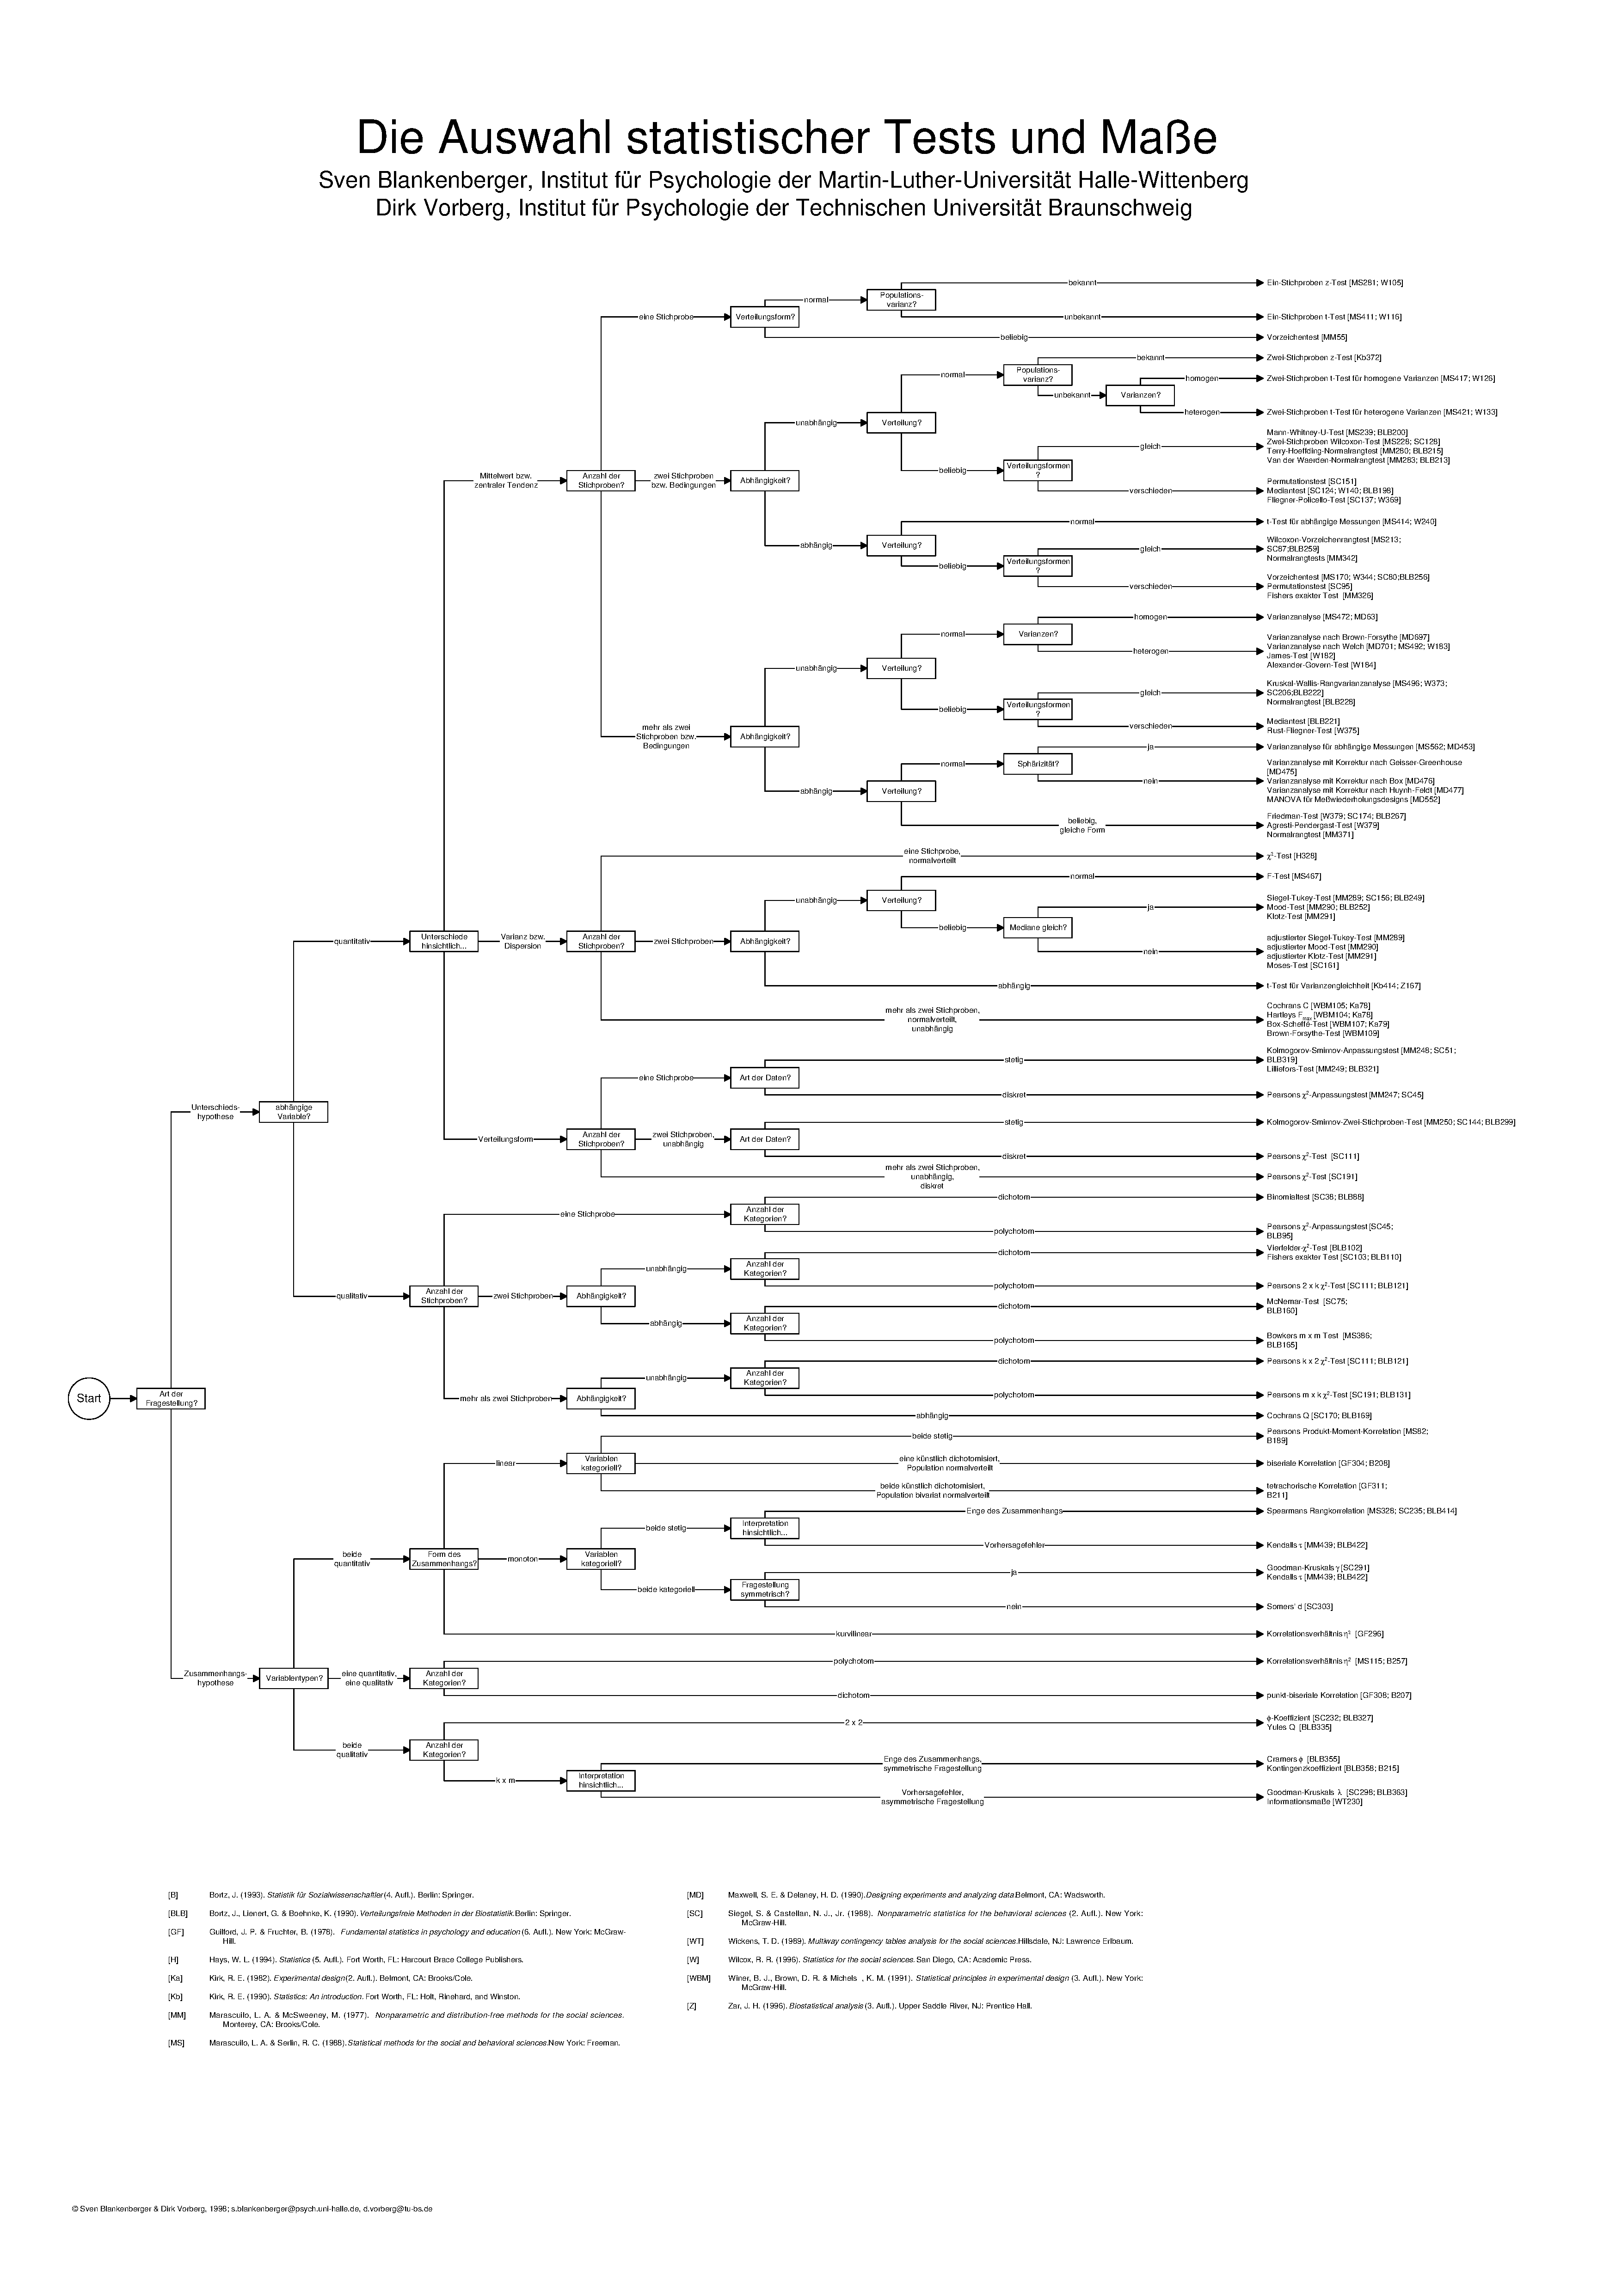
\includegraphics[width=0.7\linewidth]{img/entscheidungsbaum} 

}

\end{figure}

\href{https://md.psych.bio.uni-goettingen.de/mv/entscheidungsbaum.pdf}{Quelle}
\end{frame}

\begin{frame}{Oder man nimmt einfach immer die Regression}
\protect\hypertarget{oder-man-nimmt-einfach-immer-die-regression}{}
\begin{figure}[H]

{\centering 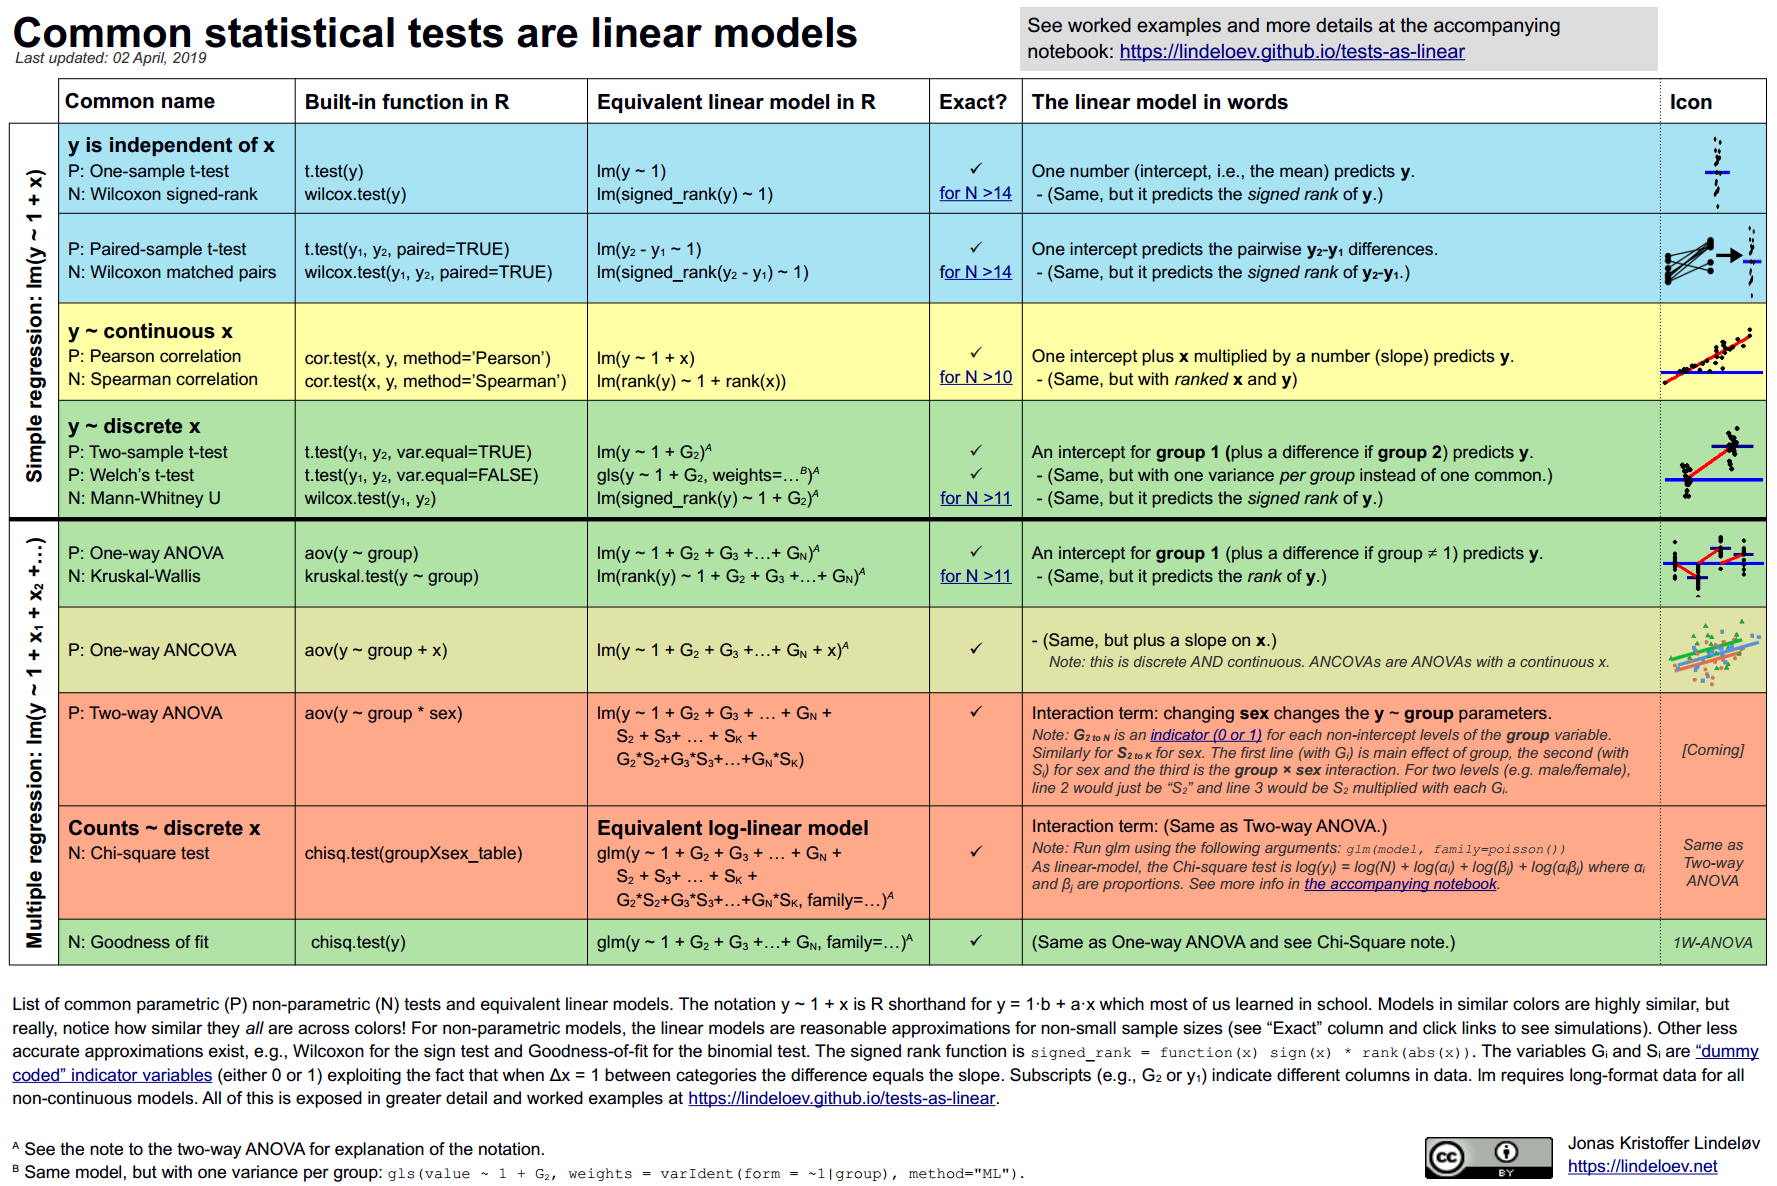
\includegraphics[width=0.7\linewidth]{img/linear_tests_cheat_sheet} 

}

\end{figure}

\href{https://lindeloev.github.io/tests-as-linear/}{Quelle}
\end{frame}

\begin{frame}{To rule 'em all}
\protect\hypertarget{to-rule-em-all}{}
\begin{figure}[H]

{\centering 
\includegraphics[width=0.5\linewidth]{img/einring} 

}

\end{figure}

\href{https://imgflip.com/i/5m9qrp}{Quelle}
\end{frame}

\begin{frame}{Was war noch mal die Regression?}
\protect\hypertarget{was-war-noch-mal-die-regression}{}
\begin{itemize}
\item
  Regression (Regressionsanalyse) ist eine Methode, um Zielvariablen in
  Abhängigkeit der Ausprägung von Prädiktorvariablen von Beobachtungen
  vorherzusagen.
\item
  Dabei erlaubt die Regression die Quantifizierung der Ungewissheit der
  Vorhersagen.
\end{itemize}

\begin{figure}[H]
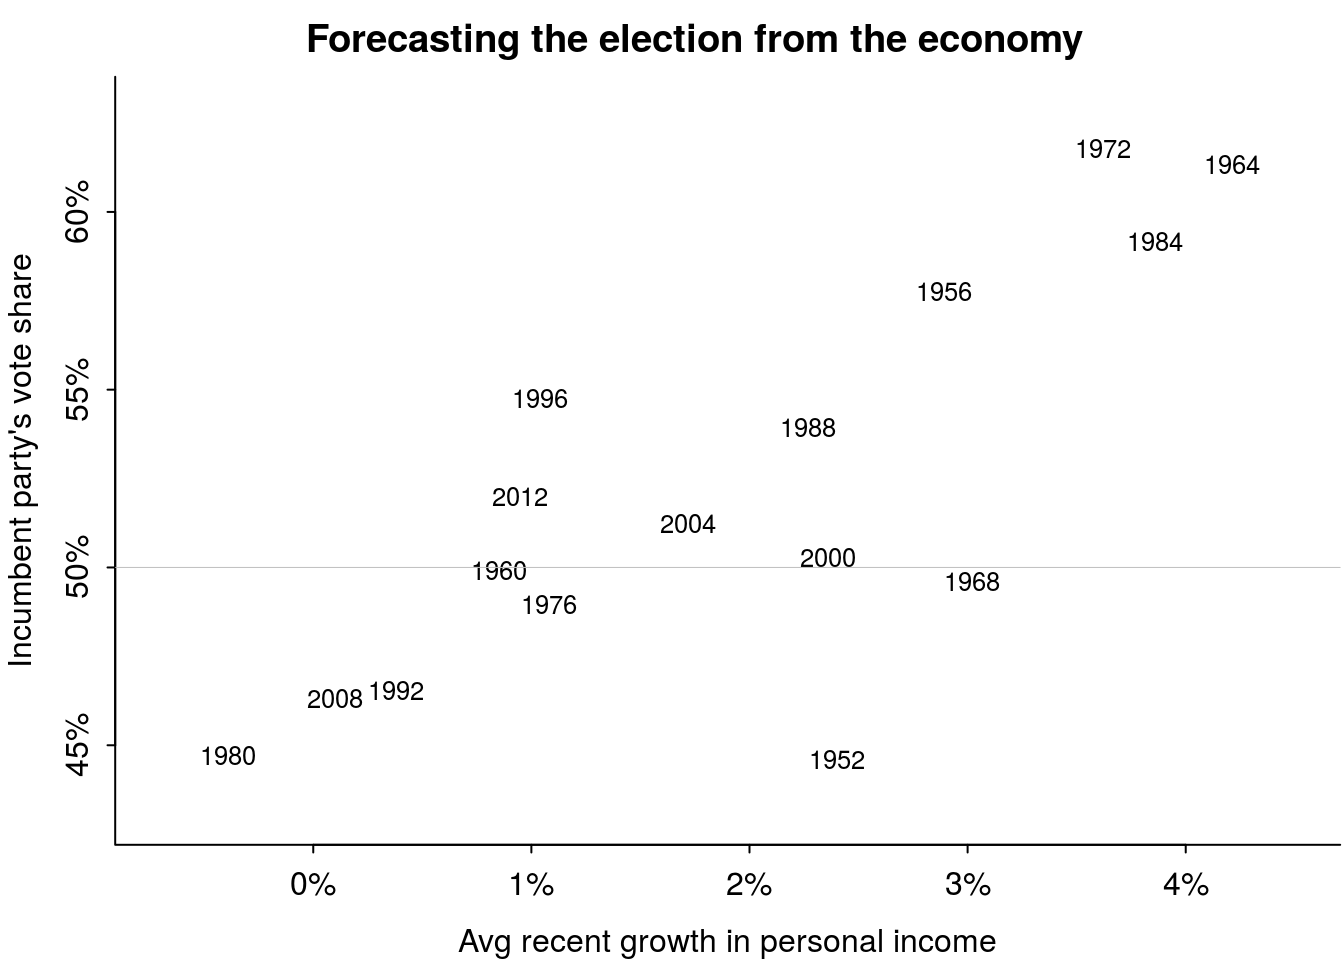
\includegraphics[width=0.4\linewidth]{img/fig1-1a} 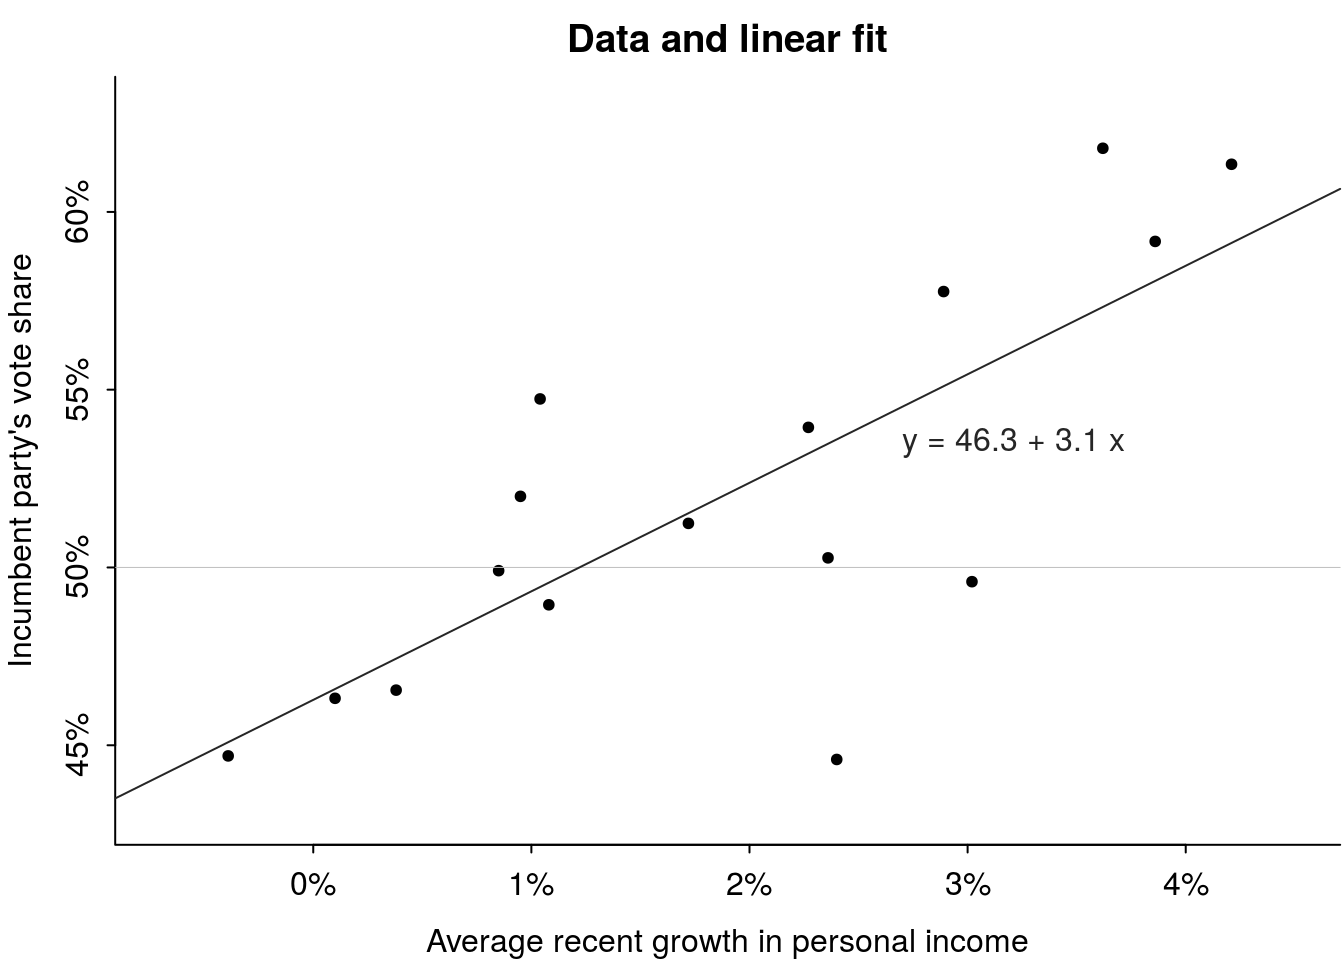
\includegraphics[width=0.4\linewidth]{img/fig1-1b} \end{figure}

\href{https://avehtari.github.io/ROS-Examples/ElectionsEconomy/hibbs.html}{Quelle}
\end{frame}

\begin{frame}{In voller Pracht: Die Regressionsgleichung}
\protect\hypertarget{in-voller-pracht-die-regressionsgleichung}{}
\[y = b_0 + b_1x + \epsilon\]

\begin{itemize}
\tightlist
\item
  \(y\): Zielvariable (vorherzusagen)
\item
  \(b_0\): Achsenabschnitt
\item
  \(b_1\): Regressionsgewicht (Steigung der Regressionsgeraden)
\item
  \(\epsilon\): ``Fehler'', Ungewissheit der Vorhersage
\end{itemize}
\end{frame}

\begin{frame}[fragile]{Datenbeispiel}
\protect\hypertarget{datenbeispiel}{}
\begin{Shaded}
\begin{Highlighting}[]
\FunctionTok{data}\NormalTok{(mtcars)}
\FunctionTok{library}\NormalTok{(rstanarm)}
\NormalTok{lm1 }\OtherTok{\textless{}{-}} \FunctionTok{stan\_glm}\NormalTok{(mpg }\SpecialCharTok{\textasciitilde{}}\NormalTok{ hp, }\AttributeTok{data =}\NormalTok{ mtcars)}
\end{Highlighting}
\end{Shaded}

\begin{Shaded}
\begin{Highlighting}[]
\FunctionTok{print}\NormalTok{(lm1)}
\end{Highlighting}
\end{Shaded}

\begin{verbatim}
            Median MAD_SD
(Intercept) 30.0    1.7  
hp          -0.1    0.0  

Auxiliary parameter(s):
      Median MAD_SD
sigma 3.9    0.5   
\end{verbatim}
\end{frame}

\begin{frame}{Visualisierung zum Datenbeispiel}
\protect\hypertarget{visualisierung-zum-datenbeispiel}{}
\begin{figure}[H]
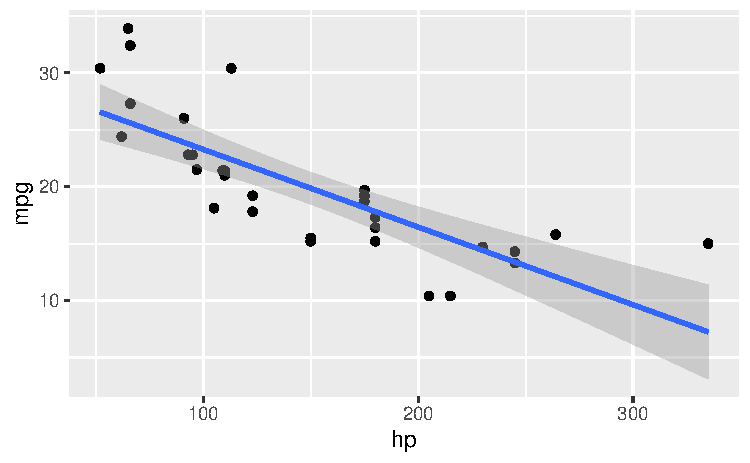
\includegraphics[width=0.7\linewidth]{unnamed-chunk-11-1} \end{figure}
\end{frame}

\begin{frame}{Wozu man die Regression benutzt}
\protect\hypertarget{wozu-man-die-regression-benutzt}{}
\begin{itemize}
\item
  Vorhersagen
\item
  Zusammenhänge untersuchen
\item
  Adjustieren (Zusammenhänge korrigieren)
\item
  Kausalinferenz
\end{itemize}
\end{frame}

\begin{frame}{In Experimenten kann man die Ergebnisse kausal
interpretieren\footnote<.->{Wenn alles gut läuft.}}
\protect\hypertarget{in-experimenten-kann-man-die-ergebnisse-kausal-interpretieren}{}
\begin{figure}[H]
\includegraphics[width=0.4\linewidth]{/Users/sebastiansaueruser/github-repos/ROS-Examples/SimpleCausal/figs/overview_1a} \includegraphics[width=0.4\linewidth]{/Users/sebastiansaueruser/github-repos/ROS-Examples/SimpleCausal/figs/overview_1b} \end{figure}
\end{frame}

\begin{frame}{Die lineare Regression ist erstaunlich flexibel}
\protect\hypertarget{die-lineare-regression-ist-erstaunlich-flexibel}{}
Z.B.

\begin{itemize}
\item
  \emph{Nichtlineare} Zusammenhänge
\item
  Interaktionen
\end{itemize}

\begin{figure}[H]
\includegraphics[width=0.4\linewidth]{/Users/sebastiansaueruser/github-repos/ROS-Examples/SimpleCausal/figs/overview_2a} \includegraphics[width=0.4\linewidth]{/Users/sebastiansaueruser/github-repos/ROS-Examples/Interactions/figs/interactions_male} \end{figure}
\end{frame}

\begin{frame}{Häufig sind Gruppen nicht direkt vergleichbar}
\protect\hypertarget{huxe4ufig-sind-gruppen-nicht-direkt-vergleichbar}{}
\begin{itemize}
\tightlist
\item
  \emph{Beispiel}: Die Heilungsraten in der Experimentalgruppe waren
  höher als in der Kontrollgruppe. Allerdings waren die Personen der
  Experimentalgrupe auch gesünder (als die Personne der Kontrollgruppe).
  Um den Kausaleffekt der Behandlung zu schätzen, müssen solche vorab
  bestehenden Unterschiede zwischen den Gruppen berücksichtigt
  (adjustiert) werden.
\end{itemize}

\begin{figure}[H]
\includegraphics[width=0.4\linewidth]{/Users/sebastiansaueruser/github-repos/ROS-Examples/SimpleCausal/figs/overview_3} \end{figure}
\end{frame}

\begin{frame}{Keine vorschnelle Kausalinterpretation}
\protect\hypertarget{keine-vorschnelle-kausalinterpretation}{}
\begin{itemize}
\tightlist
\item
  Kausalinterpretationen statistischer Ergebnisse (z.B.
  Mittelwertsdifferenz von Behandlungs- vs.~Kontrollgruppe) ist nur
  möglich, wenn

  \begin{itemize}
  \tightlist
  \item
    die Studie gut kontrolliert und randomisiert ist (und die Stichprobe
    groß ist) oder
  \item
    bestehende Unterschiede nicht randomisiert, aber kontrolliert wurden
    oder
  \item
    diese gemessen und in der Regressionsanalyse berücksichtigt wurden
  \end{itemize}
\end{itemize}

Ansonsten muss auf eine Kausalinterpretation verzichtet werden.

Allerdings ist es möglich, Art und Stärke von Zusammenhängen zu
schätzen.
\end{frame}

\hypertarget{klassische-vs.-bayes-inferenz}{%
\section{Klassische
vs.~Bayes-Inferenz}\label{klassische-vs.-bayes-inferenz}}

\begin{frame}{Klassische Inferenz: Frequentismus}
\protect\hypertarget{klassische-inferenz-frequentismus}{}
\begin{itemize}
\tightlist
\item
  Die Berücksichtigung von Vorwissen zum Sachgegenstand wird vom
  Frequentismus als subjektiv zurückgewiesen.
\item
  Nur die Daten selber fließen in die Ergebnisse ein
\item
  Wahrscheinlichkeit wird über relative Häufigkeiten definiert.
\item
  Es ist nicht möglich, die Wahrscheinlichkeit einer Hypothese
  anzugeben.
\item
  Stattdessen wird angegeben, wie häufig eine vergleichbare Datenlage zu
  erwarten ist, wenn die Hypothese gilt und der Versuch sehr häufig
  wiederholt ist.
\item
  Ein Großteil der Forschung (in den Sozialwissenschaften) verwendet
  diesen Ansatz.
\end{itemize}
\end{frame}

\begin{frame}{Bayesianische Inferenz}
\protect\hypertarget{bayesianische-inferenz}{}
\begin{itemize}
\tightlist
\item
  Vorwissen (Priori-Wissen) fließt explizit in die Analyse ein (zusammen
  mit den Daten).
\item
  \emph{Wenn} das Vorwissen gut ist, wird die Vorhersage genauer,
  ansonsten ungenauer.
\item
  Die Wahl des Vorwissens muss explizit (kritisierbar) sein.
\item
  In der Bayes-Inferenz sind Wahrscheinlichkeitsaussagen für Hypothesen
  möglich.
\item
  Die Bayes-Inferenz erfordert mitunter viel Rechenzeit und ist daher
  erst in den letzten Jahren (für gängige Computer) komfortabel
  geworden.
\end{itemize}
\end{frame}

\begin{frame}{Vergleich von Wahrscheinlichkeitsaussagen}
\protect\hypertarget{vergleich-von-wahrscheinlichkeitsaussagen}{}
\begin{columns}[T]
\begin{column}{0.48\textwidth}
\begin{block}{Frequentismus}
\protect\hypertarget{frequentismus}{}
\begin{itemize}
\item
  zentrale Statistik: \emph{p-Wert}
\item
  ``Wie wahrscheinlich ist der Wert der Teststatistik (oder noch
  extereme Werte), vorausgesetzt die Nullhypothese gilt und man
  wiederholt den Versuch unendlich oft (unter gleichen Bedingungen aber
  zufällig verschieden)?''
\end{itemize}
\end{block}
\end{column}

\begin{column}{0.48\textwidth}
\begin{block}{Bayes-Statistik}
\protect\hypertarget{bayes-statistik}{}
\begin{itemize}
\item
  zentrale Statistik: \emph{Posterior-Verteilung}
\item
  ``Wie wahrscheinlich ist die Forschungshypothese, jetzt nachdem wir
  die Daten kennen laut unserem Modell?''
\end{itemize}
\end{block}
\end{column}
\end{columns}
\end{frame}

\begin{frame}{Frequentist und Bayesianer}
\protect\hypertarget{frequentist-und-bayesianer}{}
\begin{figure}[H]
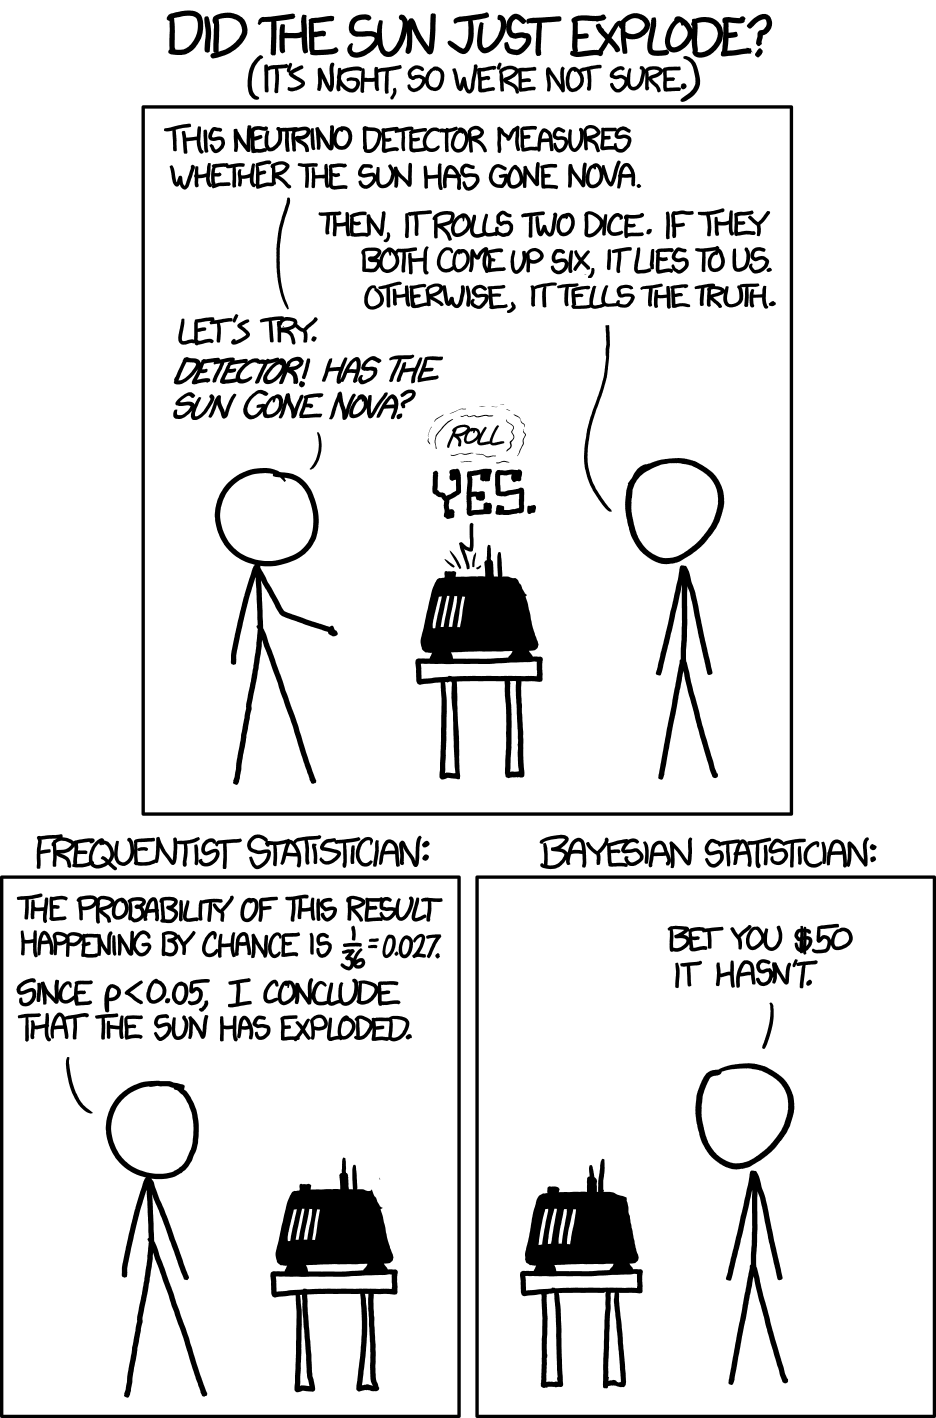
\includegraphics[width=0.7\linewidth]{img/frequentists-vs-bayesians-2x} \end{figure}

\href{https://xkcd.com/1132/}{Quelle}
\end{frame}

\begin{frame}{Beispiel zum Nutzen von Apriori-Wissen 1}
\protect\hypertarget{beispiel-zum-nutzen-von-apriori-wissen-1}{}
\begin{itemize}
\item
  Ein Betrunkener behauptet, er könne hellsehen.
\item
  Er wirft eine Münze 10 Mal und sagt jedes Mal korrekt vorher, welche
  Seite oben landen wird.
\item
  Die Wahrscheinlichkeit dieses Ergebnisses ist sehr gering
  (\(2^{-10}\)) unter der Hypothese, dass die Münze fair ist, dass
  Ergebnis also ``zufällig'' ist.
\item
  Unser Vorwissen lässt uns allerdings trotzdem an der Hellsichtigkeit
  des Betrunkenen zweifeln, so dass die meisten von uns die Hypothese
  von der Zufälligkeit des Ergebnisses wohl nicht verwerfen.
\end{itemize}
\end{frame}

\begin{frame}{Beispiel zum Nutzen von Apriori-Wissen 2}
\protect\hypertarget{beispiel-zum-nutzen-von-apriori-wissen-2}{}
\begin{itemize}
\item
  Eine Studie fand einen ``großen Effekt'' auf das Einkommen von Babies,
  eine Stunde pro Woche während zwei Jahren an einem psychosozialen
  Entwicklungsprogramm teilnahmen (im Vergleich zu einer
  Kontrollgruppe), \(n=127\).
\item
  Nach 20 Jahren war das mittlere Einkommen der Experimentalgruppe um
  42\% höher (als in der Kontrollgruppe) mit einem Konfidenzintervall
  von {[}+2\%,+98\%{]}.
\item
  Allerdings lässt uns unser Vorwissen vermuten, dass so ein Treatment
  das Einkommen nach 20 Jahren kaum verdoppeln lässt. Wir würden den
  Effekt lieber in einem konservativeren Intervall schätzen (enger um
  Null).
\end{itemize}
\end{frame}

\begin{frame}[fragile]{Regression in R, der schnelle Weg zum Glück}
\protect\hypertarget{regression-in-r-der-schnelle-weg-zum-gluxfcck}{}
\emph{Bayesianische} Inferenz in der Regression:

\begin{Shaded}
\begin{Highlighting}[]
\NormalTok{lm1 }\OtherTok{\textless{}{-}} \FunctionTok{stan\_glm}\NormalTok{(y }\SpecialCharTok{\textasciitilde{}}\NormalTok{ x, }\AttributeTok{data =}\NormalTok{ meine\_daten)}
\end{Highlighting}
\end{Shaded}

\emph{Klassische} Inferenz in der Regression:

\begin{Shaded}
\begin{Highlighting}[]
\NormalTok{lm1 }\OtherTok{\textless{}{-}} \FunctionTok{lm}\NormalTok{(y }\SpecialCharTok{\textasciitilde{}}\NormalTok{ x, }\AttributeTok{data =}\NormalTok{ meine\_daten)}
\end{Highlighting}
\end{Shaded}
\end{frame}

\hypertarget{modelle}{%
\section{Modelle}\label{modelle}}

\begin{frame}{Was ist ein (statistisches) Modell?}
\protect\hypertarget{was-ist-ein-statistisches-modell}{}
\begin{itemize}
\item
  Ein Modell ist ein vereinfachtes Abbild der Wirklichkeit, z.B. in Form
  einer Landkarte, eines Modellauto oder einer Gleichung (Sauer 2019).
\item
  Greift relevante Aspekte der Wirklichkeit heraus (und vernachlässigt
  andere).
\end{itemize}

\begin{figure}[H]
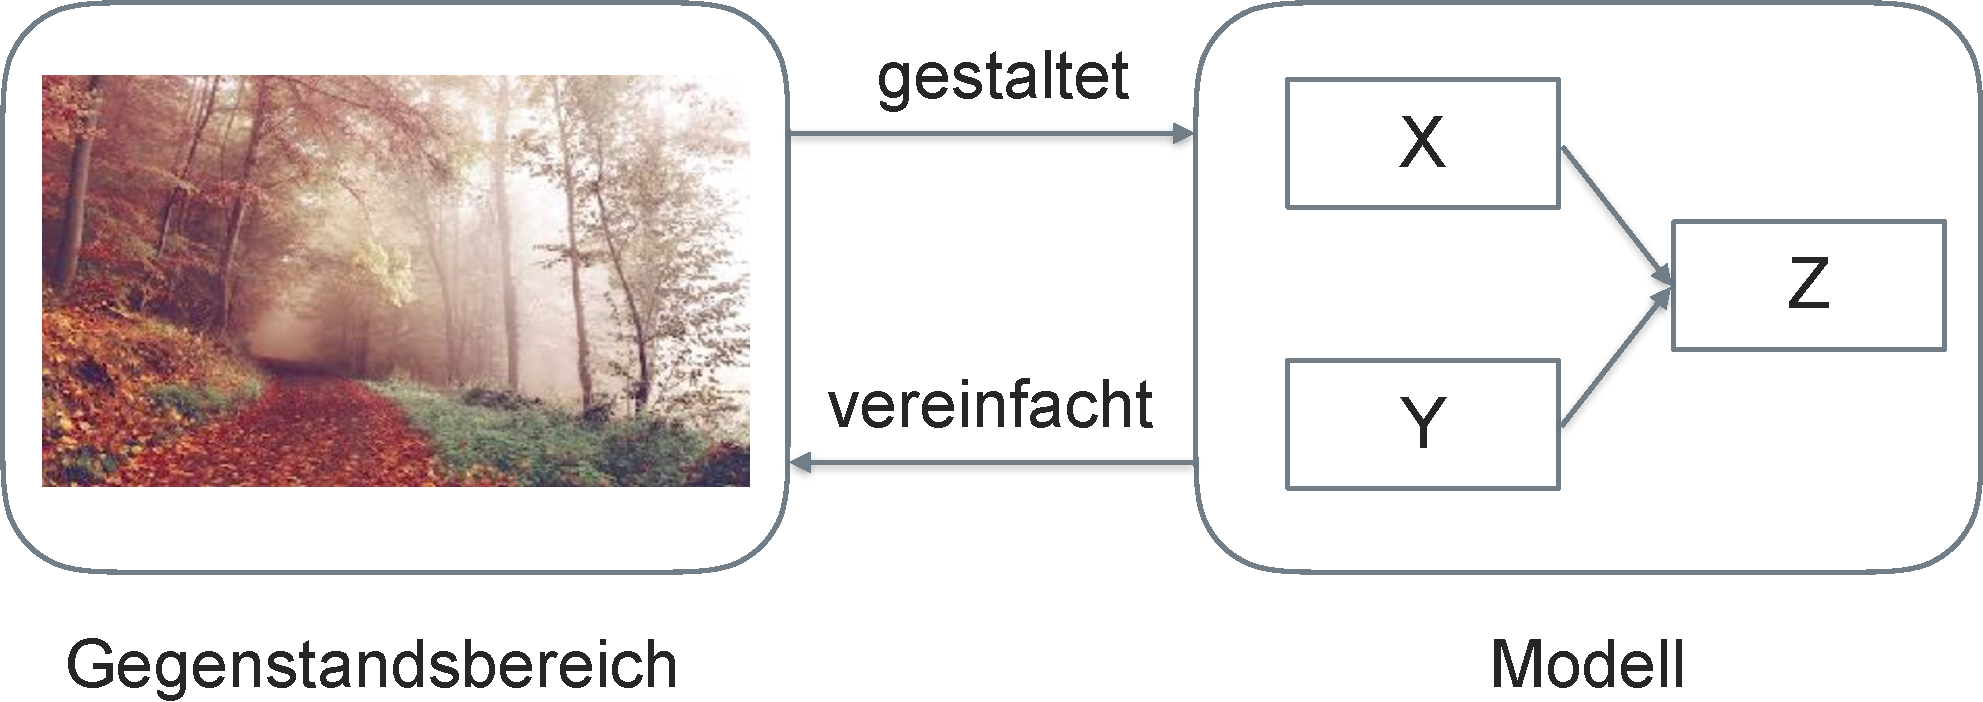
\includegraphics[width=0.7\linewidth]{img/Modell-crop} \end{figure}
\end{frame}

\begin{frame}{Beispiel für ein statistisches Modell}
\protect\hypertarget{beispiel-fuxfcr-ein-statistisches-modell}{}
\[E = \beta_0 + \beta_1\cdot L + \epsilon,\]

wobei \(E\) für \emph{Erfolg in der Klausur} steht, \(L\) für die
\emph{Lernzeit} und \(\epsilon\) für den ``Fehler'' des Modells, sprich
sonstige Einflussgrößen, die im Modell nicht berücksichtigt werden.
\end{frame}

\begin{frame}{Der Golem von Prag}
\protect\hypertarget{der-golem-von-prag}{}
\begin{columns}[T]
\begin{column}{0.5\textwidth}
\begin{figure}[H]
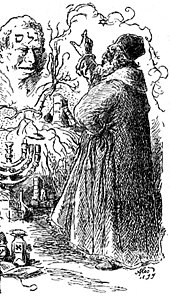
\includegraphics[width=0.5\linewidth]{img/170px-Golem_and_Loew} \end{figure}

\href{https://de.wikipedia.org/wiki/Golem}{Quelle}
\end{column}

\begin{column}{0.5\textwidth}
Der Golem von Prag, eine vom Menschen geschaffene Kreatur gewaltiger
Kraft, die Befehle wörtlich ausführt.

Bei kluger Führung kann ein Golem Nützliches vollbringen.

Bei unüberlegter Verwendung wird er jedoch großen Schaden anrichten.
\end{column}
\end{columns}
\end{frame}

\begin{frame}{Wissenschaftliche Modelle sind wie Golems}
\protect\hypertarget{wissenschaftliche-modelle-sind-wie-golems}{}
\begin{columns}[T]
\begin{column}{0.5\textwidth}
\begin{block}{Golem}
\protect\hypertarget{golem}{}
\begin{itemize}
\tightlist
\item
  Besteht aus Lehm
\item
  Belebt durch ``Wahrheit''
\item
  Mächtig
\item
  Führt Befehle wörtlich aus
\item
  Missbrauch leicht möglich
\item
  Märchen
\end{itemize}
\end{block}
\end{column}

\begin{column}{0.5\textwidth}
\begin{block}{Modell}
\protect\hypertarget{modell}{}
\begin{itemize}
\tightlist
\item
  Besteht aus \sout{Lehm}Silikon
\item
  Belebt durch Wahrheit (?)
\item
  Manchmal mächtig
\item
  Führt Befehle wörtlich aus
\item
  Missbrauch leicht möglich
\item
  Nicht einmal falsch
\end{itemize}
\end{block}
\end{column}
\end{columns}

\emph{Wir bauen Golems.}
\end{frame}

\hypertarget{hinweise}{%
\section{Hinweise}\label{hinweise}}

\begin{frame}{Lehrbuch und Homepage des Lehrbuchs}
\protect\hypertarget{lehrbuch-und-homepage-des-lehrbuchs}{}
Dieses Skript bezieht sich auf folgende
\protect\hyperlink{literatur}{Lehrbücher}:

\begin{itemize}
\item
  Kapitel 1 aus Gelman, Hill, und Vehtari (2021), \emph{Regression and
  other Stories} (mit ``ROS'' abgekürzt)
\item
  Kapitel 1 aus McElreath (2016) (``ReThink\_v1'')
\end{itemize}

Weitere Literaturhinweise sind am Ende der jeweiligen Kapitel der
Lehrbücher zu finden

R-Code zum Buch ROS findet sich auf der
\href{https://avehtari.github.io/ROS-Examples/examples.html}{Homepage}
des Buchs.
\end{frame}

\begin{frame}{Literatur}
\protect\hypertarget{literatur}{}
\hypertarget{refs}{}
\begin{CSLReferences}{1}{0}
\leavevmode\vadjust pre{\hypertarget{ref-gelman_regression_2021}{}}%
Gelman, Andrew, Jennifer Hill, und Aki Vehtari. 2021. \emph{Regression
and Other Stories}. Analytical Methods for Social Research. {Cambridge}:
{Cambridge University Press}.

\leavevmode\vadjust pre{\hypertarget{ref-McElreath2016}{}}%
McElreath, Richard. 2016. \emph{Statistical {Rethinking}}. {New York
City, NY}: {CRC Press}.

\leavevmode\vadjust pre{\hypertarget{ref-sauer_moderne_2019}{}}%
Sauer, Sebastian. 2019. \emph{Moderne Datenanalyse mit R: Daten
einlesen, aufbereiten, visualisieren und modellieren}. 1. Auflage 2019.
FOM-Edition. {Wiesbaden}: {Springer}.
\url{https://www.springer.com/de/book/9783658215866}.

\end{CSLReferences}
\end{frame}

\end{document}
